\documentclass[main.tex]{subfiles}

\theoremstyle{definition}
\newtheorem{definition}{Definition}[section]

\begin{document}
\section{Quantum world basis}
In this chapter we will build the foundations of our quantum world knowledge.
We will start from understanding some basic and very important quantum phenomena which will be 
a must-know for the following chapters. Then we will talk about the notation of quantum computing, it's basic concept and its current
state of the art.
	\subsection{Quantum phenomena}
	In this section we will discuss the most important quantum mechanics phenomena for the quantum computing world.
	Before we start we have to clarify the concept of \textit{quantum state}
	
	\theoremstyle{definition}
	\begin{definition}{\textbf{Quantum state}}
	In quantum physics, quantum state refers to the state of an isolated quantum system. A quantum state provides a probability 
	distribution for the value of each observable, i.e. for the outcome of each possible measurement on the system.
	\end{definition}
	
	\theoremstyle{definition}
	\begin{definition}{\textbf{Superposition}}
	Quantum superposition states that, much like waves in classical physics, 
	any two (or more) quantum states can be added together, \textit{superposed}, and the result will be another valid quantum state; 
	and conversely, that every quantum state can be represented as a sum of two or more other distinct states.
	\end{definition}
	
	\theoremstyle{definition}
	\begin{definition}{\textbf{Entanglement}}
	Quantum entanglement states that pairs or group of particles could be generated, interact in ways such that quantum state of a 
	single particle can't be described without describing the whole quantum system state.
	\end{definition}
		
	\subsection{Qubit}
	A quantum bit, or qubit for short, is the counterpart in quantum computing to the binary digit or bit of classical computing. 
	Just as a bit is the basic unit of information in a classical computer, a qubit is the basic unit of information 
	in a quantum computer. In a classical system, a bit would have to be in one state or the other. However, quantum mechanics allows
	the qubit to be in a coherent superposition of both states/levels simultaneously, a property which is fundamental to quantum
	mechanics and quantum computing. This property gives quantum computing a new tool to unlock new class of algorithms which are 
	more efficient.
	
		\subsubsection{Representation}
		A qubit can be represented with various notations. Each notation has its own advantage in different scenarios. 
		The main representations are the following.
		\paragraph{Standard representation}
		A qubit can be interpreted as a vector whose component are a linear superposition of its two orthonormal basis states. 
		The	basis in our case are the possible value of the qubit after its measurement, 0 or the 1 state. 
		This quantum states are usually represented with the Dirac/bra-ket notation.
		The notation uses angle brackets and a vertical bar to denote the scalar product of vectors or the action of a linear 
		functional on a vector in a complex vector space. So for example the scalar product between $v_i$ and $v_j$ can be expressed
	 	as $\braket{v_i|v_j}$; the left part $\bra{}$ is called \textit{bra} and the right part $\ket{}$ is called \textit{ket}. A
	 	ket is a representation of a single vector, so our basis can be represented as 
		\begin{center}
		$\ket{0} = 
		\begin{bmatrix}
           1 \\
           0
        \end{bmatrix},\quad
        \ket{1} = 
		\begin{bmatrix}
           0 \\
           1
        \end{bmatrix}$
		\end{center}
       	This notation is very useful for describing qubit in superposition state. We have said that a qubit can be 
        represented as a linear combination of its basis, so we can write 
      	\begin{equation}
        \ket{\psi}=\alpha\ket{0}+\beta\ket{1} 
        \quad \alpha, \beta \in \mathbb{C}
        \end{equation}
        where $\alpha$ and $\beta$ are probability amplitudes. So for the Born rule the probability of a given qubit to have 
        value $\ket{0}$ is equal to $|\alpha|^2$
        and to have value equal to $\ket{1}$ is $|\beta|^2$. Because the absolute squares of the amplitudes equate to probabilities,
        it follows that $\alpha$ an $\beta$ must be constrained by the equation
        \begin{equation}
        |\alpha|^2+|\beta|^2=1
        \end{equation}
        This notation can also describe states of multiple qubits. The quantum state of multiple qubits can be represented as tensor product between them. So for example for two qubits we have
		\begin{center}        
        $\ket{00} =
        \begin{bmatrix}
           1 \\
           0 \\
           0 \\
           0 
        \end{bmatrix}$
        ,
         $\ket{01} =
        \begin{bmatrix}
           0 \\
           1 \\
           0 \\
           0 
        \end{bmatrix}$
        ,
         $\ket{10} =
    	\begin{pmatrix}
        0\\
        1
        \end{pmatrix}
        \otimes
        \begin{pmatrix}
        1\\
        0
        \end{pmatrix}
        =
        \begin{bmatrix}
           0 \\
           0 \\
           1 \\
           0 
        \end{bmatrix}$
        ,
         $\ket{11} = 
		\begin{bmatrix}
           0 \\
           0 \\
           0 \\
           1 
         \end{bmatrix}$
        \end{center}
        
        One very important clarification has to be done. A qubit can't have a value between "0" or "1", in fact when measured its
        value can only be $\ket{0}$ or $\ket{1}$. The superposition is given by the intrinsic uncertainty of the qubit and the
        impossibility of knowing its value until measuring/collapsing it.
         
		\paragraph{Bloch sphere}
		Another frequently used notation is the Bloch sphere. This notation is based on the fact that (1) has more degrees of 
		freedom than needed, 4 degrees, so we can eliminate some of them. We start from (1)
		\begin{align*}
		\ket{\psi} 
		& =\alpha\ket{0}+\beta\ket{1} 
		& \quad\textit{standard notation}\\
        & =r_0e^{i\phi_0}\ket{0}+r_1e^{i\phi_1}\ket{1} 
        & \quad\textit{expand complex number}\\
        & =e^{i\phi_0}[r_0\ket{0}+r_1e^{i(\phi_1-\phi_0))}\ket{1}]      
        & \quad\textit{factoring }e^{i\theta_0}\\
        & =r_0\ket{0}+r_1e^{i(\phi_1-\phi_0))}\ket{1}     
        & \quad e^{i\phi_0}\textit{ is irrelevant}\\
        & =r_0\ket{0}+r_1e^{i\phi}\ket{1}    
        & \quad\textit{rename }\phi_1-\phi_0\textit{ with }\phi\\
        & =\cos{\frac{\theta}{2}}\ket{0}+\sin{\frac{\theta}{2}}e^{i\phi}\ket{1}
        & \textit{apply (2) and substitute }r_0=\cos{\frac{\theta}{2}},\quad r_1=\sin{\frac{\theta}{2}}\\
        \end{align*}
		The last equation has only two variable $\theta$ and $\phi$. We can interpret $\ket{\psi}$ as a vector in a three
		dimensional space described with polar coordinate. We only need two angle because we know that from (2) $\ket{\psi}$ 
		is a unit vector. For clarity let's make an example. If we have 
		$$\theta=0, \quad \phi=0$$
		$$\ket{\psi} = 1 \ket{0} + 0 \ket{1} = \ket{0}$$
		or another example
		$$\theta=\frac{\pi}{2}, \quad \phi=0$$
		$$\ket{\psi} = \frac{1}{\sqrt{2}} \ket{0} + \frac{1}{\sqrt{2}} \ket{1} = \ket{+}$$
		
		\begin{figure}
		\begin{center}
			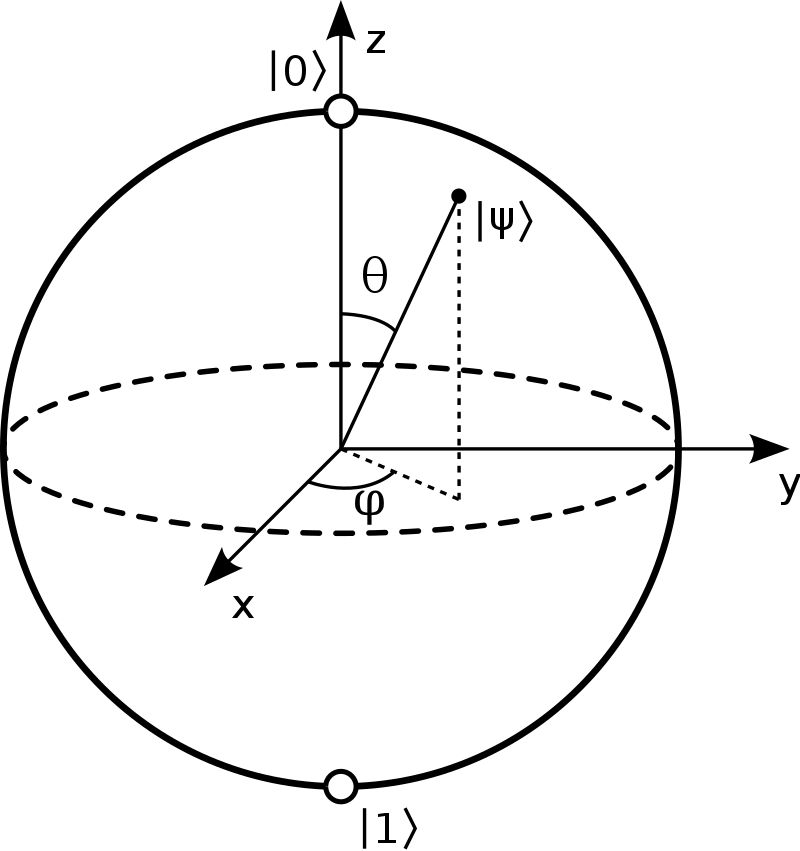
\includegraphics[scale=0.4]{Bloch_sphere.png}
			\caption{Bloch sphere. Basis states are antipodal. All intermediate states on the unitary sphere are a superposision of 
			basis states}
		\end{center}
		\end{figure}
		
		\subsubsection{Physical realization}
		In this section we will give a little introduction to the physical implementation of a qubit. Like a classical bit needs
		one physical dimension to store information, like voltage on a transistor gate, the same needs a qubit. The difference is in 
		the physical dimension used. Qubit are based on quantum property like polarization, particle spin, charge or on the presence of a 
		particle like a photon or an electron. 
		For example take a qubit based on electron spin; The spin of an electron can be in two state, \textit{up} or \textit{down}. 
		Our goal is to measure the electron spin and interpret it as a qubit.
		In practice a phosphorous atom is embedded in the p-type part of a classical n-p-n transistor.
		Then a large magnetic field is applied to the transistor. The spin of the outermost electron of the phosphorous atom will 
		align with the magnetic field in the lowest energy configuration, so the spin will tend to the down state. But there's a 
		problem, at room temperature the electron has enough energy to flip its spin to higher energy configuration, so the spin 
		would bounce between up and down state. So the system must be cool down to some hundredth of degrees above absolute zero. 
		Doing so there is not enough thermal energy to flip the spin from down to up. Now we know how to set our electron in a 
		spin down state but it would be great if we could change its spin at will. To do so we can apply microwave at specific 
		frequency, in particular at electron resonance frequency. But we can do better, if we apply the microwave for a shorter time than
		needed for transitioning from the down state to the up state, we can put the electron in a superposition state with a specific phase 
		between the two stable state. Now we know how to set the value of a qubit the only thing remaining is its measurement.
		As we have said before an electron in the up state has more energy than when it's in the down state. So when more energetic the 
		phosphorous electron can jump in the silicon leaving behind the bare phosphorous nucleus. Doing so the phosphorous nucleus will 
		have a positive charge which will be reflected in the transistor gate voltage which can be read to determine the electron spin.
	
	\subsection{Quantum computation}
	Now that we have a basic understanding of some quantum phenomena, and a representation of the minimum quantum information, a qubit, 
	we can discuss how to manipulate them in order to do some computation.
	In this document we will consider a digital approach to quantum computing, which involves quantum logic gates to do computation. 
	The opposite approach to the digital one is the analogic approach, which will not be discussed in this document.
	The digital approach consist in manipulating a n-qubit register sequentially through quantum gates.
	
	\paragraph{Quantum logic gates}Gates can be considered like a quantum equivalent of classical logic gates, but they change the 
	quantum state of the qubits manipulating their probability distribution rather than apply logic functions to the input. 
	Also quantum logic gates have to follow some restrictions that emerge from the nature of qubit. All gates must be 
	reversible, in other word the gate function must be	bijective, so from the output of the gate we can infer the input.
	This property arises from the probability nature of qubit. We know that for (2) the probability amplitudes must preserve their
	sum to 1. So every gate must conserve a coherent superposition state. To better understand how a gate can do that we can consider
	Bloch sphere. As we have said before we can interpret a qubit as a unit vector in a three dimensional space. Applying a gate is 
	equivalent to rotate the qubit vector around the origin in the Bloch sphere. So a quantum logic gate must be a unitary operation 
	in order to preserve the length of the vector. The reversibility is a property of unitary operations.\\
	
	Quantum logic gates are represented by unitary matrices. The number of qubits in the input and output of the gate must be 
	equal; a gate which acts on $n$ qubits is represented by a $2^n\text{x}2^n$ unitary matrix. The most common quantum gates operate on 
	spaces of one or two qubits, just like the common classical logic gates. The quantum states that the gates act upon are vectors 
	in $2^n$ complex dimensions. The action of the gate on a specific quantum state is found by multiplying 
	the vector $\ket{ab}$, which represent the state, by the matrix U representing the gate.
	\begin{equation}
	U\ket{ab}
	\end{equation}
	
	Now that we know which rules a quantum gate must follow, we can present the available gates.
	
	\paragraph{Hadamard gate (H)} The Hadamard gate acts on a single qubit. It's purpose is to map the
	basis state $\ket{0}$  and $\ket{1}$ to a superposition state.
	The hadamard gate is the combination of two rotation, $\pi$ about the Z-axis and 
	$\frac{\pi}{2}$ about Y-axis. 
	So it's operation matrix is
	\begin{equation}
	H=\frac{1}{\sqrt{2}}
	\begin{bmatrix}
	1 & 1\\
	1 & -1
	\end{bmatrix}
	\end{equation}
	Now let's make an example applying the H gate to the basis states.
	\begin{equation}
	H\ket{0}=\frac{1}{\sqrt{2}}
	\begin{bmatrix}
	1 & 1\\
	1 & -1
	\end{bmatrix}
	\begin{bmatrix}
	1 \\
	0
	\end{bmatrix}
	=\frac{1}{\sqrt{2}}
	\begin{bmatrix}
	1 \\
	1
	\end{bmatrix}
	=
	\frac{1}{\sqrt{2}}\ket{0}+\frac{1}{\sqrt{2}}\ket{1}
	\end{equation}
	\begin{equation}
	H\ket{1}=\frac{1}{\sqrt{2}}
	\begin{bmatrix}
	1 & 1\\
	1 & -1
	\end{bmatrix}
	\begin{bmatrix}
	0 \\
	1
	\end{bmatrix}
	=\frac{1}{\sqrt{2}}
	\begin{bmatrix}
	1 \\
	-1
	\end{bmatrix}
	=
	\frac{1}{\sqrt{2}}\ket{0}-\frac{1}{\sqrt{2}}\ket{1}
	\end{equation}
	
	
	\paragraph{Pauli X gate (X)} The Pauli-X gate acts on a single qubit. It is the quantum equivalent of the NOT gate for classical 
	computers (with respect to the standard basis states $\ket{0}$ and $\ket{1}$).  It equates to a rotation around the X-axis of the
	Bloch sphere by $\pi$ radians. Its matrix is 
	\begin{equation}
	X=
	\begin{bmatrix}
	0 & 1\\
	1 & 0
	\end{bmatrix}
	\end{equation}
	So for example if we apply it on the basis states we have
	
	$$
	X\ket{0}=
	\begin{bmatrix}
	0 & 1\\
	1 & 0
	\end{bmatrix}
	\begin{bmatrix}
	1 \\
	0
	\end{bmatrix}
	=
	\begin{bmatrix}
	0 \\
	1
	\end{bmatrix}
	=\ket{1}
	$$
	$$
	X\ket{1}=
	\begin{bmatrix}
	0 & 1\\
	1 & 0
	\end{bmatrix}
	\begin{bmatrix}
	0 \\
	1
	\end{bmatrix}
	=
	\begin{bmatrix}
	1 \\
	0
	\end{bmatrix}
	=\ket{0}
	$$
	
	\paragraph{Pauli Y gate (Y)} The Pauli-Y gate acts on a single qubit. It equates to a rotation around the Y-axis of the Bloch sphere by $\pi$ radians. So its matrix is 
	\begin{equation}
	Y=
	\begin{bmatrix}
	0 & -i\\
	i & 0
	\end{bmatrix}
	\end{equation}
	The effect of the gate is to map
	$\ket{0}$ to $i\ket{1}$ and 
	$\ket{1}$ to $-i\ket{0}$. In fact
	$$
	Y\ket{0}=
	\begin{bmatrix}
	0 & -i\\
	i & 0
	\end{bmatrix}
	\begin{bmatrix}
	1 \\
	0
	\end{bmatrix}
	=
		\begin{bmatrix}
	0 \\
	i
	\end{bmatrix}
	=
	i\ket{1}
	$$
	$$
	Y\ket{1}=
	\begin{bmatrix}
	0 & -i\\
	i & 0
	\end{bmatrix}
	\begin{bmatrix}
	0 \\
	1
	\end{bmatrix}
	=
		\begin{bmatrix}
	-i \\
	0
	\end{bmatrix}
	=
	-i\ket{0}
	$$
	
	\paragraph{Pauli Z gate (Z)} The Pauli-Z gate acts on a single qubit. It equates to a rotation around the Z-axis of the Bloch sphere by $\pi$ radians. It's equivalent to 
	a phase shift with $\phi=\pi$.
	Its matrix is
	\begin{equation}
	Z=
	\begin{bmatrix}
	1 & 0\\
	0 & -1
	\end{bmatrix}
	\end{equation}
	It's effect is to leave $\ket{0}$ unchanged and to map $\ket{1}$ to $-\ket{1}$. In fact we have
	$$
	Z\ket{0}=
	\begin{bmatrix}
	1 & 0\\
	0 & -1
	\end{bmatrix}
	\begin{bmatrix}
	1 \\
	0
	\end{bmatrix}
	=
	\begin{bmatrix}
	1 \\
	0
	\end{bmatrix}
	=
	\ket{0}
	$$
	$$
	Z\ket{1}=
	\begin{bmatrix}
	1 & 0\\
	0 & -1
	\end{bmatrix}
	\begin{bmatrix}
	0 \\
	1
	\end{bmatrix}
	=
	\begin{bmatrix}
	0 \\
	-1
	\end{bmatrix}
	=
	-\ket{1}
	$$	
	
	\paragraph{Controlled not gate (CNOT)}Controlled gates act on 2 or more qubits, where one or more qubits act as a control for some operation. For example, the controlled NOT gate (or CNOT or cX) acts on 2 qubits, and performs the NOT operation on the second qubit only when the first qubit is $\ket{1}$, and otherwise leaves it unchanged. With respect to the basis $\ket{00}, \ket{01}, \ket{10}, \ket{11}$, it is represented by the matrix:
	\begin{equation}
	CNOT=
	\begin{bmatrix}
	1 & 0 & 0 & 0\\
	0 & 1 & 0 & 0\\
	0 & 0 & 0 & 1\\
	0 & 0 & 1 & 0
	\end{bmatrix}
	\end{equation}
	So, for example
	$$
	CNOT\ket{10}=
	\begin{bmatrix}
	1 & 0 & 0 & 0\\
	0 & 1 & 0 & 0\\
	0 & 0 & 0 & 1\\
	0 & 0 & 1 & 0
	\end{bmatrix}
	\begin{bmatrix}
	0 \\
	0 \\
	1 \\
	0
	\end{bmatrix}
	= 
	\begin{bmatrix}
	0 \\
	0 \\
	0 \\
	1
	\end{bmatrix}
	=
	\ket{11}
	$$
	
	
\end{document}

\newpage
